% **************************************************************************** %
\chapter{L\"osungsans\"atze und Simulationen}
\label{chap:simu}
% **************************************************************************** %

Bevor  simuliert  werden  kann,  m\"ussen  die  daf\"ur  ben\"otigten  Modelle
vorhanden sein. In diesem Abschnitt wird zuerst ein Modell f\"ur eine PV-Zelle
bestimmt und  anschliessend benutzt,  um ein  PV-Modul aufzubauen.   Es werden
verschiedene L\"osungsans\"atze  pr\"asentiert, mit den  entwickelten Modellen
simuliert und die Resultate beurteilt.


% ---------------------------------------------------------------------------- %
\section{Modellierung einer PV-Zelle}
\label{sec:simu:model:cell}
% ---------------------------------------------------------------------------- %

\begin{wrapfigure}{r}{65mm}
    \centering
    % Simple Single-Diode Model
\begin{circuitikz}
    \footnotesize
    \draw
    % Source to top terminal
    (0,0) to[current source,i=$I_{\mathrm{Ph}}$] (0,2) -- (2,2) to[R,l^=$R_{\mathrm{S}}$] (4,2) node[ocirc] {}

    % Open terminal at bottom
    (4,0) node[ocirc] {} -- (0,0)

    % Voltage arrow over open terminals
    (4,1.7) -- (4,0.3) node[currarrow,rotate=-90] {}
    (4,1) node[anchor=west] {$V_{\mathrm{offen}}$}

    % Parallel elements
    (1,0) to[empty diode,*-*,l_=$D$] (1,2)
    (2,0) to[R,*-*,l_=$R_{\mathrm{Sh}}$] (2,2)
    ;
\end{circuitikz}

    \caption[Eindiodenmodell PV-Zelle]{%
        Eindiodenmodell  einer  PV-Zelle  mit  Stromquelle  $I_{\mathrm{Ph}}$,
        Diode  $D$,  Shunt-Widerstand $R_{\mathrm{Sh}}$~  und  Seriewiderstand
        $R_{\mathrm{S}}$.%
    }
    \label{fig:pvcell:1diode}
\end{wrapfigure}

Das Modell  einer idealien  Photovoltaikzelle ist  eine Stromquelle  mit einer
parallel geschalteten Diode. Da PV-Zellen in Realit\"at nicht ideal sind, wird
das einfachste Ersatzschaltbild einer PV-Zelle \"ublicherweise durch einen zur
Stromquelle parallel geschalteten Shunt-Widerstand $R_{\mathrm{Sh}}$ und einen
Seriewiderstand $R_{\mathrm{S}}$ erg\"anzt; das resultierende Ersatzschaltbild
ist in Abbildung \ref{fig:pvcell:1diode} dargestellt.

Die Genauigkeit  dieses Eindiodenmodells  ist jedoch h\"aufig  nicht besonders
gut  \cite{pvcell:phang}  \cite{pvcell:masmoudi}   (besonders  bei  niederigen
Beleuchtungsgraden),   weshalb   wir   hier  ein   Zweidiodenmodell   benutzen
werden. Eine  der  beiden  Dioden   modelliert  dabei  den  S\"attigungsstrom,
welcher von  Diffusionsprozessen verursacht wird, die  zweite Diode modelliert
den  S\"attigungsstrom,  welcher  von Rekombinationseffekten  verursacht  wird
\cite{pvcell:masmoudi}.

Zur Herleitung der Modellparamater existieren verschiedene Verfahren. Man kann
beispielsweise eine  PV-Zelle im Labor  ausmessen und die  Modellparameter aus
diesen  Messergebnissen  ableiten.   Dies  ist jedoch  nicht  immer  praktisch
realisierbar, da man allenfalls kein Testexemplar zur Verf\"ugung hat.  Sollen
bei  der  Messung  noch Fertigungstoleranzen  der  PV-Zellen  ber\"ucksichtigt
werden,  steigt der  experimentelle  (und  finanzielle) Aufwand  zus\"atzlich,
da  man  mehrere Exemplare  kaufen  und  ausmessen muss. Auch  die  Auswertung
erfordert mehr Arbeit, wenn  man mittels statistischer Methoden verl\"assliche
Schlussfolgerungen ziehen k\"onnen will.

Alternativ   kann   man   auch   versuchen,  die   Modellparameter   aus   dem
Datenblatt  einer  PV-Zelle  herzuleiten. Dies  bietet  zwei  haupts\"achliche
Vorteile: Einerseits  entfallen  aufw\"andige  Messungen   und  der  Kauf  von
Testexemplaren, andererseits ist davon auszugehen, dass der Hersteller mehrere
Exemplare ausgemessen hat  und typische Angaben in  den Datenbl\"atten gemacht
werden.  Es setzt jedoch voraus,  dass man den Herstellerangaben einigermassen
vertraut;  Sicherheit  ist  letztendlich  nur  durch  eigene  Verifikation  zu
erlangen.

Das Herleiten der Modellparameter aus den Herstellerangaben ist nicht trivial;
es wird deshalb  an dieser Stelle ein Modell  einer kommerziell erh\"altlichen
PV-Zelle  \todo{Hersteller   nennen}  als  Grundlage  verwendet,   welches  in
\cite{pvcell:masmoudi} hergeleitet und verifiziert worden ist.

\"Ublicherweise wird  bei PV-Zellen  nur das  Gleichstromverhalten untersucht;
das Verhalten  unter Wechselstrom interessiert meistens  nicht. Da das Signal,
welches  in  diesem  Projekt  auf die  DC-Leitung  aufmoduliert  wird,  jedoch
Wechselstrom ist,  sollte das  Wechselstromverhalten von PV-Zellen  in unseren
Simulationen ber\"ucksichtigt werden.

Das  Zweidiodenmodell  aus  \cite{pvcell:masmoudi}  wird  deshalb  in  unseren
Simulationen   noch   durch    eine   parallele   Kapazit\"at   erg\"anzt. Die
Gr\"ossenordnung   dieser   Kapazit\"at   kann  stark   variieren   und   wird
unter    anderem   vom    Diodenmaterial,   der    Diodenspannung   und    der
Diodentemperatur   beeinflusst. Basierend    auf   \cite{capacitance:hegedus},
\cite{capacitance:mandal}     und      \cite{capacitance:mauk}     soll     an
dieser    Stelle   eine    fl\"achennormierte    Kapazit\"at    von   $C'    =
\SI{20}{\nano\farad\per\centi\meter\squared}$    verwendet   werden. Die    in
\cite{pvcell:masmoudi}    verwendete    Zelle    hat   eine    Gr\"osse    von
$\SI{125}{\milli\meter}    \times     \SI{125}{\milli\meter}$    (allf\"allige
abgeschnittene  Ecken, wie  sie in  Abbildung \ref{fig:pvcell:front}  zu sehen
sind,  werden  vernachl\"assigt),  womit  die  Kapazit\"at  einer  Zelle  sich
berechnet zu:

\begin{equation}
    \label{eq:capa:jac}
    C_{\mathrm{Zelle}}
    = A_{\mathrm{Zelle}} \cdot C'
    = \left( \SI{125}{\milli\meter} \right)^4 \cdot \SI{20}{\nano\farad\per\centi\meter\squared}
    = \SI{3.125}{\micro\farad}
\end{equation}

Somit  sind das  Ersatzschaltbild  und die  zugeh\"origen Parameter  bestimmt;
die  Ergebnisse  sind  in Abbildung  \ref{fig:circuit:solarCell}  und  Tabelle
\ref{tab:solarCell:params} abgebildet respektive aufgelistet.
\todo{referenz spice}

\begin{figure}[h!tb]
    \centering
    % Parametrized version, can be put at coordinates x and y
%
%\newcommand{\CTSolarCell}[2]{%
%    % Source to top terminal
%    (0+#1,0+#2) to[current source,i=$I_{\mathrm{Zelle}}$] (0+#1,4+#2) -- (5+#1,4+#2) to[R,l^=$R_{\mathrm{S}}$] (10+#1,4+#2) node[circ] {}
%
%    % Open terminal at bottom
%    (10+#1,0+#2) node[circ] {} -- (0+#1,0+#2)
%
%    % Voltage arrow over open terminals
%    %(10+#1,3.7+#2) -- (10+#1,0.3+#2) node[currarrow,rotate=-90] {}
%    %(10+#1,2+#2) node[anchor=west] {$V_{\mathrm{offen}}$}
%
%    % Parallel elements
%    (1.5+#1,4+#2) to[empty diode,*-*,l_=$D$] (1.5+#1,0+#2)
%    (3+#1,4+#2) to[C,*-*,l_=$C$] (3+#1,0+#2)
%    (4.5+#1,4+#2) to[R,*-*,l_=$R_{\mathrm{P}}$] (4.5+#1,0+#2)%
%}


% Single Diode
%\begin{circuitikz}
%    \draw
%    % Source to top terminal
%    (0,0) to[current source,i=$I_{\mathrm{Zelle}}$] (0,3) -- (5,3) to[R,l^=$R_{\mathrm{S}}$] (8,3) node[ocirc] {}
%
%    % Open terminal at bottom
%    (8,0) node[ocirc] {} -- (0,0)
%
%    % Voltage arrow over open terminals
%    (8,2.7) -- (8,0.3) node[currarrow,rotate=-90] {}
%    (8,1.5) node[anchor=west] {$V_{\mathrm{offen}}$}
%
%    % Parallel elements
%    (1.5,3) to[empty diode,*-*,l_=$D$] (1.5,0)
%    (3,3) to[C,*-*,l_=$C$] (3,0)
%    (4.5,3) to[R,*-*,l_=$R_{\mathrm{P}}$] (4.5,0)
%    ;
%\end{circuitikz}

% Two Diodes
\begin{circuitikz}
    \draw
    % Source to top terminal
    (0,0) to[current source,i=$I_{\mathrm{Ph}}$] (0,3) -- (7.5,3) to[R,l^=$R_{\mathrm{S}}$] (11,3) node[ocirc] {}

    % Open terminal at bottom
    (11,0) node[ocirc] {} -- (0,0)

    % Voltage arrow over open terminals
    (11,2.7) -- (11,0.3) node[currarrow,rotate=-90] {}
    (11,1.5) node[anchor=west] {$V_{\mathrm{offen}}$}

    % Parallel elements
    (2,3) to[empty diode,*-*,l_=$D_{\mathrm{Diff}}$] (2,0)
    (4.5,3) to[empty diode,*-*,l_=$D_{\mathrm{Rekomb}}$] (4.5,0)
    (6,3) to[C,*-*,l_=$C$] (6,0)
    (7.5,3) to[R,*-*,l_=$R_{\mathrm{Sh}}$] (7.5,0)
    ;
\end{circuitikz}

    \caption[Zweidiodenmodell PV-Zelle mit zus\"atzlicher Kapazit\"at]{%
        Schaltschema    zur    Modellierung    einer    Solarzelle    gem\"ass
        Zweidiodenmodell  mit  zus\"atzlicher  Kapazit\"at. Die  zugeh\"origen
        Modellparameter    sind    in    Tabelle    \ref{tab:solarCell:params}
        aufgelistet.%
    }
    \label{fig:circuit:solarCell}
\end{figure}

\begin{table}[h!t]
    \centering
    \caption{\"Ubersicht Modellparameter f\"ur Solarzelle aus Abbildung \ref{fig:circuit:solarCell}}
    \label{tab:solarCell:params}
    \begin{tabular}{llrp{20mm}}
        \toprule
        Parameter                              & Symbol                  & Wert                       & Quelle                 \\
        \midrule
        Diodenstrom (\emph{Photo Current})     & $I_{\mathrm{Ph}}$       & \SI{5.889}{\ampere}        & \cite{pvcell:masmoudi} \\
        S\"attigungsstrom Diffusionsdiode      & $I_{\mathrm{S,Diff}}$   & \SI{794.06}{\pico\ampere}  & \cite{pvcell:masmoudi} \\
        S\"attigungsstrom Rekombinationsdiode  & $I_{\mathrm{S,Rekomb}}$ & \SI{5.0762}{\micro\ampere} & \cite{pvcell:masmoudi} \\
        Idealit\"atsfaktor Diffusionsdiode     & $n_{\mathrm{Diff}}$     & \num{1}                    & \cite{pvcell:masmoudi} \\
        Idealit\"atsfaktor Rekombinationsdiode & $n_{\mathrm{Rekomb}}$   & \num{2}                    & \cite{pvcell:masmoudi} \\
        Seriewiderstand                        & $R_{\mathrm{S}}$        & \SI{1.71}{\milli\ohm}      & \cite{pvcell:masmoudi} \\
        Shunt-Widerstand                       & $R_{\mathrm{Sh}}$       & \SI{59.23}{\ohm}           & \cite{pvcell:masmoudi} \\
        Kapazit\"at                            & $C$                     & \SI{3.125}{\micro\farad}   & \cite{capacitance:hegedus}, \cite{capacitance:mandal}, \cite{capacitance:mauk}, Gl. \ref{eq:capa:jac} \\
        Kantenl\"ange                          & $s$                     & \SI{125}{\milli\meter}     & \cite{pvcell:masmoudi} \\
        \bottomrule
    \end{tabular}
\end{table}

% ---------------------------------------------------------------------------- %
\clearpage
\section{Modellierung eines PV-Moduls}
\label{sec:simu:model:module}
% ---------------------------------------------------------------------------- %


Das im obigen Abschnitt hergeleitete PV-Zellen-Modell wird nun dazu verwendet,
ein Modell f\"ur ein  PV-Modul aufzubauen. In Anhang \ref{app:models:calcs} ab
Seite  \pageref{app:models:calcs}  sind  als Anhaltspunkt  die  Daten  einiger
kommerzieller PV-Module mit verschiedenen Zellenkonfigurationen aufgelistet.

Es     wird    ein     PV-Modul     aus    72     in    Serie     angeordneten
Zellen    gew\"ahlt     und    implementiert. Es    wird     ebenfalls    eine
Freilaufdiode    parallel    zu     jedem    Modul    geschaltet,    basierend
auf     den      in     Abbildungen     \ref{fig:simu:iv-curves:array:generic}
\ref{fig:simu:iv-curves:array:generic:bypass}   gezeigten  Effekten   und  den
zugeh\"origen Anmerkungen.

\begin{wrapfigure}{l}{50mm}
    \centering
    \begin{tikzpicture}
    \begin{scope}[x={(0mm,50mm)},y={(0mm,-80mm)},line width=1pt,cap=round]

        \node[anchor=north west,inner sep=0pt] at (0,0) {%
            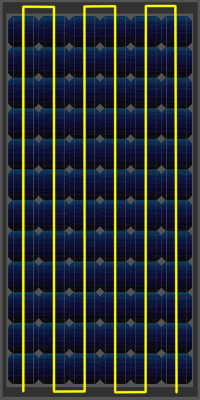
\includegraphics[width=40mm,height=80mm]{images/solar-facility/pvmodule-wiring.jpeg}
        };

        % Horizontal Measurement (Wires)
        % ==============================

        % Horizontal measurement between wires
        \draw (5mm,0mm) -- (5mm,4mm); % Vertical line
        \draw (11mm,0mm) -- (11mm,4mm);   % Vertical line

        % Measurement arrow
        \draw[-latex] (4mm,2mm) -- (5mm,2mm);
        \draw[-] (4mm,2mm) -- (31.5mm,2mm);
        \draw[latex-] (11mm,2mm) -- (12mm,2mm);

        % Measurment
        \node[anchor=west] at (12mm,3.75mm) {\small$d = \SI{127}{\milli\meter}$};


        % Vertical measurement (Wires)
        % ============================
        \draw (4mm,-1.5mm) -- (-4mm,-1.5mm); % horizontal line
        \draw (4mm,-78.5mm) -- (-4mm,-78.5mm); % horizontal line

        \draw[latex-latex] (-2mm,-1.5mm) -- (-2mm,-78.5mm); % measurement line

        % Measurement
        \node[rotate=90] at (-3.75mm,-38.5mm) {\small$l = \SI{1550}{\milli\meter}$};

        \node at (5mm,-82.5mm) {\small 1};
        \node at (11mm,-82.5mm) {\small 2};
        \node at (17mm,-82.5mm) {\small 3};
        \node at (23mm,-82.5mm) {\small 3};
        \node at (29mm,-82.5mm) {\small 2};
        \node at (35.5mm,-82.5mm) {\small 1};
    \end{scope}
\end{tikzpicture}


    \caption[PV-Modul, Modell f\"ur den Strompfad]{
        Solarmodul  gem\"ass Abbildung  \ref{fig:pvmodule} mit  Stromleitungen
        und  L\"angen   zur  Verbindung   der  Zellen. Die   Nummerierung  der
        Leiterbahnen   entspricht    der   Nummerierung    der   Koeffizienten
        in   Gleichungen   \ref{eq:rosa:a1}    bis   \ref{eq:rosa:a3}   (Seite
        \pageref{eq:rosa:a1}).%
    }
    \label{fig:pvmodule:wiring}
    \vspace*{-3em}
\end{wrapfigure}

Der  Pfad, den  der Strom  in  einem Modul  zur\"ucklegt, kann  je nach  Modul
mehrere Meter L\"ange  erreichen.  Dieser Effekt wird in  unserem Modell durch
eine Stromleitung modelliert, die \"uber  alle Zellen geht. In Realit\"at sind
die Leiter, welche die Zellen miteinander verbinden, ziemlich kurz (angenommen
die Zellen werden  von Kante zu Kante verbunden), aber  da der Strompfad durch
die ganze Zelle geht, wird der gesamte Strompfad in underem Modell vereinfacht
als eine lange Leitung dargestellt.

Zwischen   diesen   parallelen    Leiterbahnen   ergeben   sich   parasit\"are
Induktivit\"aten, die  im Folgenden  bestimmt und  in unser  Modell integriert
werden.  Die  angenommene Form und  die Abmessungen der  internen Stromleitung
sind  in  Abbildung   \ref{fig:pvmodule:wiring}  dargestellt. Die  Abmessungen
basieren auf folgenden Annahmen:

\begin{itemize}
    \tightlist
    \item
        Kantenl\"ange eines Moduls: \SI{125}{\milli\meter}
    \item
        Abstand zwischen zwei Modulen: \SI{2}{\milli\meter}
    \item
        \"Uberhang      am      oberen      und     unteren      Ende      des
        Moduls: \SI{14}{\milli\meter}
    \item
        Der Abstand zweier Leiterbahnen ist somit \SI{127}{\milli\meter} und
    \item
        die     L\"ange     einer     Leiterbahn     summiert     sich     auf
        \SI{1550}{\milli\meter}.
\end{itemize}


Zur  Berechnung  der  parasit\"aren  Induktivit\"at wird  \emph{The  Self  and
Mutual  Inductances  of Linear  Conductors}  von  Edward B. Rosa  herangezogen
\cite{ref:inductance:rosa}. Darin  wird   unter  anderem   die  Induktivit\"at
einer   Leiterkonfiguration  wie   sie  in   unserem  Modul   angenommen  wird
(Abbildung  \ref{fig:pvmodule:wiring}) bestimmt. Die  zugeh\"orige Formel  ist
in  Gleichung  \ref{eq:rosa:snake}  gegeben\footnotemark.
\footnotetext{%
    Die  Formeln  in   \cite{ref:inductance:rosa}  sind  im  \emph{CKG}-System
    (Centimeter,    Kilogramm,    Sekunden)     notiert,    f\"ur    Gleichung
    \ref{eq:rosa:snake} ist die Gleichung von  Rosa auf das SI-System normiert
    worden.%
}

\noindent Der  Wert f\"ur die Selbstinduktivit\"at  der verschiedenen Dr\"ahte
ist nicht  identisch; dies wird im  Summand $A_{\mathrm{i}}$ ber\"ucksichtigt,
der abh\"angt von der Anzahl  paralleler Leiterbahnen und ihrer Lage innerhalb
der  Leiteranordnung. F\"ur \num{6}  parallele Leiterbahnen  ergeben sich  die
Werte aus Gleichungen \ref{eq:rosa:a1}, \ref{eq:rosa:a2} und \ref{eq:rosa:a3}.


\begin{alignat}{2}
    \label{eq:rosa:snake}
    L &= \frac{\mu_{\mathrm{0}} \cdot l}{2 \cdot \pi}
    \cdot
    \left[
        \ln\left(
            \frac{d}{\rho}
        \right)
        + \frac{1}{4}
        - A_{\mathrm{i}}
    \right] & \quad \text{Selbstinduktivit\"at eines Leiters}
    \\
    \label{eq:rosa:a1}
    A_{\mathrm{1}} &= -\ln\left(\frac{15}{8}\right) & \text{\"ausserste Leiterbahnen} \\
    \label{eq:rosa:a2}
    A_{\mathrm{2}} &= \ln\left(\frac{16}{5}\right)  & \text{Leiterbahnen Nr. 2} \\
    \label{eq:rosa:a3}
    A_{\mathrm{3}} &= \ln\left(\frac{4}{3}\right)   & \text{Leiterbahnen Nr. 3, Mitte}
\end{alignat}

\begin{conditions}
    d              & Abstand zwischen zwei Leiterbahnen \\
    \rho           & Radius des Leiters \\
    A_{\mathrm{i}} & Korrektursummand f\"ur Leiterposition gem\"ass Abbildung \ref{fig:pvmodule:wiring} \\
\end{conditions}

Somit kann f\"ur  jeder Teil der Leitung in einem  Modul dessen Induktivit\"at
berechnet  werden. Diese  werden  anschliessend summiert  (Serieschaltung  von
Induktivit\"aten) und  als Gesamtinduktivit\"at  eines Moduls in  unser Modell
integriert.

Es   wird  von   einem   Leiterquerschnitt  von   \SI{4}{\milli\meter\squared}
ausgegangen,  was  einen   Leiterradius  $\rho$  von  \SI{1.128}{\milli\meter}
ergibt.

Die  Induktivit\"aten der  Leiterbahnen  innerhalb des  Moduls k\"onnen  somit
bestimmt werden:

\begin{alignat}{2}
    L_{\mathrm{1}} &= \frac{\mu_{\mathrm{0}} \cdot l}{2 \cdot \pi}
    \cdot
    \left[
        \ln\left(
            \frac{d}{\rho}
        \right)
        + \frac{1}{4}
        - A_{\mathrm{1}}
    \right]
    & = \SI{1.737}{\micro\henry} \\
    L_{\mathrm{2}} &= \frac{\mu_{\mathrm{0}} \cdot l}{2 \cdot \pi}
    \cdot
    \left[
        \ln\left(
            \frac{d}{\rho}
        \right)
        + \frac{1}{4}
        - A_{\mathrm{2}}
    \right]
    & = \SI{1.181}{\micro\henry} \\
    L_{\mathrm{3}} &= \frac{\mu_{\mathrm{0}} \cdot l}{2 \cdot \pi}
    \cdot
    \left[
        \ln\left(
            \frac{d}{\rho}
        \right)
        + \frac{1}{4}
        - A_{\mathrm{3}}
    \right]
    & = \SI{1.453}{\micro\henry}
\end{alignat}

\begin{conditions}
    \mu_{\mathrm{0}} = 4 \cdot \pi \cdot 10^{-7} & magnetische Permeabilit\"at des Vakuums \\
    l                = \SI{1550}{\milli\meter}   & L\"ange einer Leiterbahn                \\
    d                = \SI{127}{\milli\meter}    & Abstand zweier Leiterbahnen             \\
    \rho             = \SI{1.128}{\milli\meter}  & Radius des Leiters                      \\
    A_{\mathrm{1}}   =  -0.6286                  & Korrektursummand                        \\
    A_{\mathrm{2}}   =   1.1632                  & Korrektursummand                        \\
    A_{\mathrm{3}}   =   0.2877                  & Korrektursummand                        \\
\end{conditions}

Die Gesamtinduktivit\"at der Leiterbahnen in einem Modul ist somit:

\begin{equation}
    \label{eq:pvmodule:totalInductance}
    \underline{\underline{L_{\mathrm{Modul}}
    =
    2 \cdot \left(
        L_{\mathrm{1}} + L_{\mathrm{2}} + L_{\mathrm{3}}
    \right)
    = \SI{8.74}{\micro\henry}}}
\end{equation}

Es bleibt noch der Ohm'sche Widerstand der Leiterbahn zu bestimmen\footnotemark.
Dieser errechnet sich zu:

\footnotetext{%
    Es  sei  an   dieser  Stelle  darauf  hingewiesen,  dass   der  im  Modell
    der  Solarzelle  vorkommende  Seriewiderstand $R_{\mathrm{S}}$  nicht  die
    Leiterbahnen modelliert, sondern thermische Verluste im Halbleitersubstrat
    \cite{pvcell:masmoudi}%
}

\begin{equation}
    \label{eq:resistance:ohm:module}
    \underline{\underline{R = \frac{\rho \cdot l}{A} = \SI{44.2}{\milli\ohm}}}
\end{equation}

\begin{conditions}
    A = \SI{4}{\milli\meter\squared} & Querschnittsfl\"ache des Leiters \\
    \rho = \SI{0.0178}{\ohm\milli\meter\squared\per\meter} & Spezifischer Widerstand Leitungskupfer \cite{ref:kuchling:rhoCu} \\
    l = (6 \cdot 1550 + 5 \cdot 127)\si{\milli\meter} = \SI{9.935}{\meter} & Gesamtl\"ange des Leiters in einem Modul \\
\end{conditions}

Mit  diesen Informationen  kann  das Schaltbild  f\"ur  ein PV-Modul  bestimmt
werden,  was  die  Schaltung  in  Abbildung  \ref{fig:circuit:72x1:simplified}
ergibt. Dieses  Modell  wird im  Folgenden  benutzt,  um eine  Solaranlage  zu
modellieren.

\begin{figure}[h!tb]
    \centering
    % x: 0, 1, 3, 4
\def\POSxUp{0,3}
\def\POSxDown{1,4}
\def\POSy{0,1,3,4}
\begin{circuitikz}
    \foreach \x in \POSxUp{
        \foreach \y in \POSy {
            \draw
            (\x,\y) to[empty photodiode] (\x,\y+1)
            ;
        }
        \draw (\x,2.5) node[rotate=90] {\ldots};
    }
    \foreach \x in \POSxDown{
        \foreach \y in \POSy {
            \draw
            (\x,\y+1) to[empty photodiode] (\x,\y)
            ;
        }
        \draw (\x,2.5) node[rotate=90] {\ldots};
    }

    % Connecting Lines between Strings
    \draw (0,5) -- (1,5);
    \draw (1,0) -- (3,0);
    \draw (3,5) -- (4,5);

    \draw (0,0) -- (0,-0.5) node[ocirc] {~~IN};
    \draw (4,0) -- (4,-0.5) node[ocirc] {~~OUT};
\end{circuitikz}

    \caption[Ersatzschaltbild PV-Modul]{%
        Ersatzschaltbild  f\"ur  das  PV-Modul. Es besteht  einem  Strang  mit
        72  Zellen  in Serie  geschaltet  und  angeordnet  wie auf  dem  Modul
        in  Abbildung  \ref{fig:pvmodule}  auf  Seite  \pageref{fig:pvmodule}.
        Zus\"atzlich  ist  die  parasit\"are Induktivit\"at  der  Leiterbahnen
        im  Modul ber\"ucksichtigt  und  eine  Freilaufdiode integriert.   Die
        vollst\"andige  \code{LTspice}-Schaltung  ist  in Abbildung  TODO  auf
        Seite TODO dargestellt.%
    }
    \label{fig:circuit:72x1:simplified}
\end{figure}



% ---------------------------------------------------------------------------- %
\section{Modellierung eines Modulstrangs}
\label{sec:simu:model:module:string}
% ---------------------------------------------------------------------------- %

Der zu  simulierende Modulstrang soll  aus 20  Modulen bestehen, die  in Serie
miteinander  verbunden werden. Die  Induktivit\"at der  Leitungen, welche  die
Module  miteinander verbinden,  wird  vernachl\"assigt,  da die  zugeh\"origen
Distanzen  zwischen den  Leitern viel  gr\"osser sind,  als die  Distanzen der
Leiterbahnen innerhalb eines Moduls (siehe vorheriger Abschnitt).

Es  soll  jedoch  die  Induktivit\"at  der  Anschlussleitung  ber\"ucksichtigt
werden. Dabei   soll  von   einem   \SI{20}{\meter}  langen   Doppelleiterpaar
ausgegangen  werden, das  in einem  Abstand von  \SI{20}{\milli\meter} verlegt
worden ist. Dies ist nat\"urlich eine  idealisierte Annahme; in der Realit\"at
sind  diese Leiter  weder mit  konstant gleichem  Abstand noch  perfekt gerade
verlegt.

Die  von   Rosa  in  \cite{ref:inductance:rosa}  gegebene   Formel  f\"ur  die
Induktivit\"at eines geraden, parallelen Leiterpaares lautet\footnotemark:

\footnotetext{%
    Auch  hier  ist  Rosa's  Formel  auf  das  moderne  SI-System  konvertiert
    worden. Zudem wird  davon ausgegangen,  dass die  Leiter aus  Kupfer sind.
    Dessen  relative  Permeabilit\"at  $\mu_{\mathrm{r}}$  liegt  bei  etwa  1
    \cite{ref:kuchling:muRCu} und kann somit in der Gleichung vernachl\"assigt
    werden.

    Auch Kuchling gibt in \cite{ref:Kuchling:Ltwo} die gleiche Formel.%
}

\begin{equation}
    \label{eq:rosa:dualwire}
    \underline{\underline{L = \frac{\mu_{0}}{\pi} \cdot \left[ \ln\left(\frac{d}{\rho}\right) + \frac{1}{4} \right]
    = \SI{25}{\micro\henry}}}
\end{equation}

\begin{conditions}
    \mu_{\mathrm{0}} = 4 \cdot \pi \cdot 10^{-7} & magnetische Permeabilit\"at des Vakuums \\
    l                = \SI{20}{\meter}           & L\"ange des Leiterpaares (ein Weg)    \\
    d                = \SI{20}{\milli\meter}     & Abstand der Leiter                    \\
    \rho             = \SI{1.128}{\milli\meter}  & Radius des Leiters                    \\
\end{conditions}

Da zwei parallel  verlaufende Leiter im Prinzip  einen Kondensator darstellen,
soll  an  dieser  Stelle  auch   die  parasit\"are  Kapazit\"at  der  zu-  und
wegf\"uhrenden Leiterbahnen ber\"ucksichtigt werden. Die Formel zur Berechnung
dieser Kapazit\"at ist gem\"ass Kuchling \cite{ref:Kuchling:CTwo}:

\begin{equation}
    \label{eq:rosa:dualwire}
    \underline{\underline{C = \frac{\pi \cdot \epsilon_{0} \cdot \epsilon_{\mathrm{r}} \cdot l}{\ln\left(\frac{d}{\rho}\right)}
    = \SI{193.5}{\pico\farad}}}
\end{equation}

\begin{conditions}
    \epsilon_{0} = \SI{8.854}{\pico\farad\per\meter} & Elektrische Feldkonstante          \\
    \epsilon_{\mathrm{r}} = 1                        & Permittivit\"atszahl von Luft      \\
    l                = \SI{20}{\meter}               & L\"ange des Leiterpaares (ein Weg) \\
    d                = \SI{20}{\milli\meter}         & Abstand der Leiter                 \\
    \rho             = \SI{1.128}{\milli\meter}      & Radius des Leiters                 \\
\end{conditions}

Der Ohm'sche Widerstand der Anschlussleitung errechnet sich zu:

\begin{equation}
    \label{eq:resistance:ohm:module}
    \underline{\underline{R = \frac{\rho \cdot l}{A} = \SI{178}{\milli\ohm}}}
\end{equation}

\begin{conditions}
    A    = \SI{4}{\milli\meter\squared} & Querschnittsfl\"ache des Leiters \\
    \rho = \SI{0.0178}{\ohm\milli\meter\squared\per\meter} & Spezifischer Widerstand Leitungskupfer \cite{ref:kuchling:rhoCu} \\
    l    = \SI{40}{\meter} & Gesamtl\"ange der Anschlussleitung (beide Wege) \\
\end{conditions}

\begin{figure}[h!tb]
    \centering
    \def\POSx{9,8,7,6,5,4,3,2,1,0}
%\def\POSxRight{2,3,4,5,6,7,8,9,10,11}
\begin{circuitikz}
    %(12,0) -- (10,0)

    % Right to Left
    \foreach \x in \POSx {
        \draw
        (\x,1.5) to[empty photodiode] (\x - 1,1.5)
        ;
    }

    % Left to Right
    \foreach \x in \POSx {
        \draw
        (\x-1,-1.5) to[empty photodiode] (\x,-1.5)
        ;
    }

    % Endpoints
    \draw (-1,1.5) -- (-1,-1.5);

    % Stuff on the right
    \draw (9,1.5)  -- (9,0.75)  to[L,l^=L] (12,0.75)  node[ocirc] { };
    \draw (9,-1.5) -- (9,-0.75) to[R,l_=R] (12,-0.75) node[ocirc] { };
    \draw (9.5,0.75) node[circ] { } to[C,l^=C] (9.5,-0.75) node[circ] { };
\end{circuitikz}

    \caption[Ersatzschaltbild Modulstrang mit Verbindungsleitung]{
        Modell  eines Modulstrangs  aus  20 seriell  geschalteten Modulen  mit
        Ber\"ucksichtigung der Resistivit\"at,  Induktivit\"at und Kapazit\"at
        einer \SI{20}{\meter} langen Zuleitung%
    }
    \label{fig:pvstring}
\end{figure}

Abbildung  \ref{fig:pvstring} zeigt  das  Ersatzschaltbild eines  Modulstrangs
aus    20   in    Serie   geschalteten    Modulen   mit    den   parasit\"aren
Leiterimpedanzen. Dieses  und  die  vorangegangenen   Modelle  werden  nun  in
\code{LTspice} implementiert und f\"ur Simulationen benutzt.


% ---------------------------------------------------------------------------- %
\section{Induktive Einkopplung}
\label{sec:simu:coupling:inductive}
% ---------------------------------------------------------------------------- %

Eine induktive Einkopplung legt eine  Spule um die DC-Leitung. Auf diese Spule
wird vom Sensor  das zu \"ubertragende Signal gegeben und  die Spule induziert
in der DC-Leitung entsprechende  Spannungs-Rippel, die vom \Master ausgewertet
werden k\"onnen. Der  entsprechende Schaltkreis  ist schematisch  in Abbildung
\ref{fig:circuit:coupling:inductive} dargestellt.

\code{LTspice}    modelliert   diese    Situation   als    gekoppelte   Spulen
mit    je     einer    Induktivit\"at     (L1    und    L2     in    Abbildung
\ref{fig:circuit:coupling:inductive)}und  einem   Kopplungsfaktor  K. Es  gilt
also, diese drei Parameter zu bestimmen.

Wir  werden   f\"ur  unsere   Simulationen  von  einer   Toroidspule  gem\"ass
Abbildung  \ref{fig:toroid:geometry}  mit   20  Prim\"arwicklungen  und  einer
Sekund\"arwindung (die DC-Leitung) ausgehen.  Die relative Permeabilit\"at von
ferromagnetischen Materialien  kann enorm  stark variieren; Werte  von einigen
Dutzend bis zu  mehreren Tausend k\"onnen auftreten. Wir  werden f\"ur unseren
Kern eine Permeabilit\"atszahl $\mu_{\mathrm{r}} = 400$ annehmen.

\clearpage
\begin{figure}[h!tb]
    \centering
    \begin{circuitikz}
    \draw
    (-1,0) to[empty photodiode,o-,l_=PV-Modul] (1,0) to[short] (6,0)
    %(2,-2) to[short,o-] (2,-0.05) to[L=L] (4,-0.05) to[short,-o] (4,-2)
    (2,-2) -- (2,-0.05) to[L,l^=Kopplung] (4,-0.05) -- (4,-2) to[sinusoidal voltage source,l^=$U_{\mathrm{Signal}}$] (2,-2)
    ;
\end{circuitikz}

    \caption[Prinzip der induktiven Einkopplung]{Induktive Einkopplung}
    \label{fig:circuit:coupling:inductive}
\end{figure}


Die Selbstinduktivit\"at unserer Toroidspule errechnet sich gem\"ass:

\begin{equation}
    \label{eq:selfInductance:toroid:primary}
    L_{\mathrm{1}} = \frac{\mu_{0} \mu_{\mathrm{r}} r^2 N_1^2}{2 R} \approx \SI{200}{\micro\henry}
\end{equation}

%\begin{figure}[h!tb]
\marginpar{%
    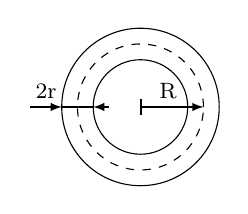
\begin{tikzpicture}
    \footnotesize
    \begin{scope}[x={(0mm,0.9\textwidth)},y={(0mm,30mm)}]
        \draw (0mm,0mm) circle[radius = 6mm];
        \draw (0mm,0mm) circle[radius = 10mm];
        \draw[dashed] (0mm,0mm) circle[radius = 8mm];
        \draw[|-latex] (0mm,0mm) -- (8mm,0mm);
        \draw (3.5mm,2mm) node {R};
        \draw[-latex] (-14mm,0mm) -- (-10mm,0mm);
        \draw (-12mm,2mm) node {2r};
        \draw (-10mm,0mm) -- (-6mm,0mm);
        \draw[latex-] (-6mm,0mm) -- (-4mm,0mm);
    \end{scope}
\end{tikzpicture}

    \figcaption[Geometrie Kopplungsspule]{\protect\raggedright Geometrie der Spule}
    \label{fig:toroid:geometry}%
}
%\end{figure}

\begin{conditions}
    \mu_0 = 4 \cdot \pi \cdot 10^{-7} & magnetische Permeabilit\"at des Vakuums               \\
    \mu_{\mathrm{r}} = 400 & angenommene relative magnetische Permeabilit\"at des Kerns       \\
    r = \SI{4}{\milli\meter} & Radius des Kernquerschnitts (Abb. \ref{fig:toroid:geometry})  \\
    R = \SI{8}{\milli\meter} & mittlerer Radius des Toroids (Abb. \ref{fig:toroid:geometry}) \\
    N_1 = 20 & Anzahl Windungen \\
\end{conditions}

Die Induktivit\"at der sekund\"aren Seite berechnet sich gem\"ass:

\begin{equation}
    \label{eq:selfInductance:toroid:secondary}
    L_{\mathrm{2}} = L_{1} \cdot \frac{N_2^2 }{N_1^2} \approx \SI{500}{\nano\henry}
\end{equation}

\begin{conditions}
    L_{\mathrm{1}} = \SI{200}{\micro\henry}
    & Selbstinduktivit\"at der Prim\"arseite (Gl. \ref{eq:selfInductance:toroid:primary})\\

    N_1 = 20 & Windungsn Prim\"arseite (Transmitter/Receiver) \\
    N_2 = 1  & Windungen Sekund\"arseite (DC-Leitung) \\
\end{conditions}

Der Kopplungsfaktor beschreibt, wie gross  der Anteil des magnetischen Flusses
ist, welcher beide Spulen durchfliesst. Ein Kopplungsfaktor von null bedeutet,
dass die  beiden Spulen  v\"ollig entkoppelt sind,  ein Kopplungsfaktor  von 1
heisst, dass der gesamte Fluss, welcher  die eine Spule durchfliesst, auch die
andere Spule durchfliesst.  Es wird  hier ein Streuverlust von 5\% angenommen,
was einen Kopplungsfaktor von 0.95 ergibt.

Es  wird   zuerst  eine  vereinfachte  Schaltung   untersucht,  bestehend  aus
einem  Modul,  dem  Sender  und  dem  Empf\"anger,  dargestellt  in  Abbildung
\ref{fig:ltspice:inductive:singleModule}.

\begin{figure}[h!tb]
    \centering
    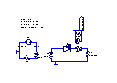
\includegraphics[width=0.67\textwidth]{images/ltspice/jac/inductive-singleModule.eps}
    \caption[Induktive Einkopplung, vereinfachte \code{LTspice}-Schaltung]{%
        \code{LTspice}-Schaltung f\"ur den vereinfachten Schaltkreis zur
        Simulation der induktiven Einkopplung%
    }
    \label{fig:ltspice:inductive:singleModule}
\end{figure}

Abbildung  \ref{fig:simu:inductive:singleModule}  zeigt  den  Spannungsverlauf
am      Empf\"anger      f\"ur      die      Schaltung      aus      Abbildung
\ref{fig:ltspice:inductive:singleModule}. Das Signal kommt sauber an, ist aber
nicht sehr stark.

\begin{figure}[h!tb]
    \begin{tikzpicture}
    %\begin{scope}[x={(0mm,0mm)},y={(175mm,\textwidth)}] % for four plots
    \begin{scope}[x={(0mm,0.95\textwidth)},y={(0mm,50mm)}]
        \begin{axis}[%
                title=Spannung am Empf\"anger,
                %title=$R_{\mathrm{Last}}$
                height=50mm,
                width=0.95\textwidth,
                at={(0,0)},
                grid=both,
                xlabel=Zeit (\si{\micro\second}),
                ylabel=Spannung (\si{\milli\volt}),
                change x base=true,
                change y base=true,
                x SI prefix=micro,
                y SI prefix=milli,
                xmin = 0,
                xmax = 10e-6,
                %legend cell align = left,
                %legend style={at={(125mm,-10mm)},anchor=north east},
           ]
           \addplot[-,blue] table[x = time,y = V(receiver)] {data/inductive/inductive-singleModule.dat};
        \end{axis}
   \end{scope}
\end{tikzpicture}

    \caption[Simulationsergebniss induktive Einkopplung, vereinfachte Schaltung]{%
        Simulationsergebniss f\"ur die Spannung am Empf\"anger aus Abbildung
        \label{fig:ltspice:inductive:singleModule}%
    }
    \label{fig:simu:inductive:singleModule}
\end{figure}

Zur  Simulation eines  ganzen Modulstrangs  wird die  Schaltung aus  Abbildung
\ref{fig:ltspice:inductive:complete}  benutzt; der  Modulstrang basiert  dabei
auf den Herleitungen aus Abschnitt \ref{Modellierung eines Modulstrangs}.

\begin{figure}[h!tb]
    \centering
    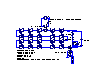
\includegraphics[width=0.95\textwidth]{images/ltspice/jac/inductive.eps}
    \caption[Induktive Einkopplung, \code{LTspice}-Schaltung f\"ur Modulstrang]{%
        Schaltung  zur   Simulation  eines  Modulstranges   mit  parasit\"aren
        Impedanzen in der Zuleitung und komplexer Lastimpedanz.%
    }
    \label{fig:ltspice:inductive:complete}
\end{figure}

\begin{figure}[h!tb]
    \begin{tikzpicture}
    %\begin{scope}[x={(0mm,0mm)},y={(175mm,\textwidth)}] % for four plots
    \begin{scope}[x={(0mm,0.95\textwidth)},y={(0mm,50mm)}]
        \begin{axis}[%
                title=Spannung am Empf\"anger{,} variierende Lastimpedanzen,
                height=50mm,
                width=0.95\textwidth,
                at={(0,0)},
                grid=both,
                xlabel=Zeit (\si{\micro\second}),
                ylabel=Spannung (\si{\milli\volt}),
                change x base=true,
                change y base=true,
                x SI prefix=micro,
                y SI prefix=milli,
                xmin = 0,
                xmax = 10e-6,
           ]
           \addplot[-,blue] table[x = time,y = V(receiver)] {data/inductive/inductive-CloadRload-stepped.dat};
        \end{axis}
   \end{scope}
\end{tikzpicture}

    \caption[Simulationsergebniss, induktive Einkopplung, Modulstrang]{%
        Simulationsergebniss f\"ur die Spannung am Empf\"anger aus Abbildung
        \ref{fig:ltspice:inductive:complete}%
    }
    \label{fig:simu:inductive:stepping}
\end{figure}

Abbildung  \ref{fig:simu:inductive:stepping}  enth\"alt  Simulationsergebnisse
f\"ur    verschiedene   Lastimpedanzen    bei    einer   Senderfrequenz    von
\SI{1}{\mega\hertz}.   Die zugeh\"origen Impedanzkombinationen sind in Tabelle
\ref{tab:inductive:stepping:params}  aufgelistet. Simulationen  mit  h\"oheren
resistiven  Anteilen w\"aren  interessant, allerdings  hat \code{LTspice}  bei
weiterem  Ansteigen von  \code{Rload} (vermutlich  numerische) Schwierigkeiten
und  die Simulationszeit  steigt auf  Tage bis  Wochen (falls  sie \"uberhaupt
jemals endet und  die Software nicht in einem Kreis  von nicht konvergierenden
Bedingungen festh\"angt).

Es  ist  zu   erkennen,  dass  das  Signal  am   Empf\"anger  nicht  besonders
stark  von  der  Lastimpedanz abh\"angt. Allerdings  ist  die  Signalamplitude
ziemlich  klein  und betr\"agt  nur  einige  Millivolt. Positiv gewertet  kann
aber  werden,  dass  das  Signal   trotz  der  kleinen  Amplitude  immer  noch
sehr  sauber  aussieht. Allerdings kann  es  nat\"urlich  sein, dass  sonstige
St\"orungseffekten   auf  der   Leitung  (welche   in  der   Simulation  nicht
ber\"ucksichtigt  worden  sind)  das Signal  \"uberdecken  w\"urden. Dies  ist
allerdings  im Rahmen  dieses  Projektes nicht  wirklich  zu verifizieren,  da
wir  weder einen  gen\"ugend grossen  Modulstrang noch  die zur  gr\"undlichen
Untersuchung erforderliche Zeit zur Verf\"ugung haben.


\begin{table}[h!tb]
    \centering
    \caption{%
        Lastimpedanzparameter  f\"ur die  Simulationsergebnisse aus  Abbildung
        \ref{fig:simu:inductive:stepping}
    }
    \label{tab:inductive:stepping:params}
    \begin{tabular}{rr|rr|rr}
        \toprule
        \code{Cload}             & \code{Rload} & \code{Cload}             & \code{Rload}  & \code{Cload}             & \code{Rload} \\
        \midrule
        \SI{  1}{\nano\farad}    & \SI{1}{\ohm} & \SI{  1}{\nano\farad}    & \SI{10}{\ohm} & \SI{  1}{\nano\farad}    & \SI{50}{\ohm} \\
        \SI{ 10}{\nano\farad}    & \SI{1}{\ohm} & \SI{ 10}{\nano\farad}    & \SI{10}{\ohm} & \SI{ 10}{\nano\farad}    & \SI{50}{\ohm} \\
        \SI{100}{\nano\farad}    & \SI{1}{\ohm} & \SI{100}{\nano\farad}    & \SI{10}{\ohm} & \SI{100}{\nano\farad}    & \SI{50}{\ohm} \\
        \SI{  1}{\micro\farad}   & \SI{1}{\ohm} & \SI{  1}{\micro\farad}   & \SI{10}{\ohm} & \SI{  1}{\micro\farad}   & \SI{50}{\ohm} \\
        \SI{ 10}{\micro\farad}   & \SI{1}{\ohm} & \SI{ 10}{\micro\farad}   & \SI{10}{\ohm} & \SI{ 10}{\micro\farad}   & \SI{50}{\ohm} \\
        \SI{100}{\micro\farad}   & \SI{1}{\ohm} & \SI{100}{\micro\farad}   & \SI{10}{\ohm} & \SI{100}{\micro\farad}   & \SI{50}{\ohm} \\
        \bottomrule
    \end{tabular}
\end{table}

Interessant    ist    der    Betrieb    des    Senders    mit    Eigenfrequenz
(ca. \SI{240}{\kilo\hertz} in diesem  Fall) des Modulstrangs\footnotemark. Der
zugeh\"orige    Spannungsverlauf    am    Empf\"anger   ist    in    Abbildung
\ref{fig:simu:inductive:resonance}   abgebildet. Hier    wird   ein   vielfach
gr\"osserer  Signalpegel  erreicht;  allerdings  ben\"otigt  das  Signal  etwa
\SI{100}{\micro\second},  bis  es wirklich  seine maximale  Amplitude erreicht
hat. Da  bei  diesem System  jedoch  keine  sehr hohen  Datenraten  ben\"otigt
werden, muss dies nicht unbedingt kritisch sein.

\footnotetext{%
    Die Eigenfrequenz  ist hier nicht  mathematisch bestimmt, sondern  aus den
    Simulationen abgelesen worden.%
}

\begin{figure}[h!tb]
    \begin{tikzpicture}
    %\begin{scope}[x={(0mm,0mm)},y={(175mm,\textwidth)}] % for four plots
    \begin{scope}[x={(0mm,0mm)},y={(50mm,\textwidth)}]
        \begin{axis}[%
                title=Spannung am Empf\"anger bei Eigenfrequenz,
                %title=$R_{\mathrm{Last}}$
                height=50mm,
                width=\textwidth,
                at={(0,0)},
                grid=both,
                xlabel=Zeit (\si{\micro\second}),
                ylabel=Spannung (\si{\milli\volt}),
                change x base=true,
                change y base=true,
                x SI prefix=micro,
                y SI prefix=milli,
                xmin = 0,
                xmax = 200e-6,
                %legend cell align = left,
                %legend style={at={(125mm,-10mm)},anchor=north east},
           ]
           \addplot[-,blue] table[x = time,y = V(receiver)] {data/inductive/inductive-resonance.dat};
        \end{axis}
   \end{scope}
\end{tikzpicture}

    \caption[Simulationsergebniss induktive Einkopplung bei Resonanz]{%
        Simulationsergebniss f\"ur die Spannung am Empf\"anger aus Abbildung
        \ref{fig:ltspice:inductive:complete}%
    }
    \label{fig:simu:inductive:resonance}
\end{figure}


Abschliessend kann man  zur induktiven Kopplung sagen, dass  sie bei kleineren
Aufbauten  gut  funktionieren  sollte,   dass  aber  bei  gr\"osseren  Anlagen
m\"oglicherweise  zus\"atzliche  Massnahmen  n\"otig sein  k\"onnten,  um  das
Signal klar empfangen und auswerten  zu k\"onnen. Dies k\"onnte z.B. bedeuten,
dass  unser System  die Eigenfrequenz  des Modulstrangs  selbst ausmisst,  und
sich entsprechend  selbst konfiguriert,  um stets  auf der  optimalen Frequenz
\"ubermitteln zu k\"onnen.


% ---------------------------------------------------------------------------- %
\clearpage
\section{Kapazitive Einkopplung}
\label{sec:simu:coupling:capacitive}
% ---------------------------------------------------------------------------- %

Bei der  kapazitiven Einkopplung  wird eine  Signalquelle via  Kondensator mit
der  DC-Leitung  verbunden. Bei  jedem  Modul und  am  Ende  des  Modulstrangs
ist   dabei  eine   Einkopplung   vorgesehen. Das   Prinzip  ist   schematisch
in   Abbildung   \ref{fig:circ:coupling:capacitive}   dargestellt. F\"ur   die
nachfolgenden  Versuche  wird  eine Tr\"agerfrequenz  von  \SI{1}{\mega\hertz}
angenommen, sofern nicht anders angegeben.

Sowohl \Master ~wie auch \Sensor~ k\"onnen dabei Signale senden und empfangen;
das Verfahren ist bidirektional.

\begin{figure}[h!tb]
    \centering
    \begin{circuitikz}
    \draw
    (0,0) to[empty photodiode,o-,l_=PV-Modul] (1,0) to[short] (10,0) node[ocirc] { }

    (3,0) node[circ] { } to[C,l^=Kopplung] (3,-1.5) to[sinusoidal voltage source,l^=$U_{\mathrm{Sender}}$] (3,-3) node[sground] { }

    (9,0) node[circ] { } to[C,l^=Kopplung] (9,-1.5) -- (9,-3) node[ocirc] {~~$U_{\mathrm{Receiver}}$};
    ;
\end{circuitikz}

    \caption[Ersatzschaltbild kapazitive Einkopplung]{%
        Vereinfachte Darstellung  der kapazitiven  Einkopplung mit  Sender auf
        der linken  Seite und  Empf\"anger auf der  rechten Seite. Prinzipiell
        ist das Verfahren jedoch bidirektional.%
    }
    \label{fig:circ:coupling:capacitive}
\end{figure}

Zur   Simulation   in  \code{LTspice}   wird   die   Schaltung  in   Abbildung
\ref{fig:ltspice:capacitive:string} benutzt. Sie basiert  auf dem Modell eines
Modulstrangs von Abbildung  \ref{fig:pvstring} (Seite \pageref{fig:pvstring}),
erg\"anzt  um  die  Ein-  und  Auskopplungsschaltung. Zus\"atzlich  wurde  eine
komplexe Lastimpedanz eingebaut.

Es werden der Signalpegel am Empf\"anger bei zwei verschiedenen Senderpositionen
untersucht: Eine zu Beginn des Strangs, eine am Ende des Strangs. Ist der Sender
am Anfang des Strangs positioniert, muss das Signal durch alle restlichen Module,
um an den Empf\"anger zu gelangen; es ist hier allenfalls mit Verzerrungen und/oder
Abschw\"achungen des Signals zu rechnen.


\begin{figure}[h!tb]
    \centering
    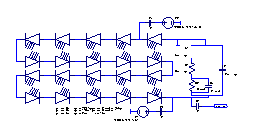
\includegraphics[width=0.75\textwidth]{images/ltspice/jac/capacitive.eps}
    \caption[\code{LTspice}-Schaltung kapazitive Einkopplung, Modulstrang]{%
        Simulationsschaltung  eines Modulstrangs  mit kapazitiver  Einkopplung
        eines  Signals. Jedes   Modulsymbol  repr\"asentiert dabei  ein  Modul
        gem\"ass  Abbildung \ref{fig:ltspice:jac:Module}  im Anhang  auf Seite
        \pageref{fig:ltspice:jac:Module}  mit Freilaufdiode  und parasit\"aren
        Leitungsimpedanzen.\protect\\
        Die  Sender  werden  durch  Sinus-Spannungsquellen  simuliert. Es  ist
        jeweils  nur ein  Sender  aktiv  in der  Simulation,  der andere  wird
        abgeh\"angt.%
    }
    \label{fig:ltspice:capacitive:string}
\end{figure}

Die    in    \code{LTspice}    benutzte    Schaltung    ist    in    Abbildung
\ref{fig:ltspice:capacitive:string}      gezeigt.       Die      zugeh\"origen
Simulationsresultate   sind    in   Abbildung   \ref{fig:simu:capacitive:tran}
zu sehen.%

\begin{figure}[h!tb]
    \begin{tikzpicture}
    %\begin{scope}[x={(0mm,0mm)},y={(175mm,\textwidth)}] % for four plots
    \begin{scope}[x={(0mm,0mm)},y={(90mm,\textwidth)}]
        \begin{axis}[%
                title=$R_{\mathrm{Last}} {=} \SI{1}{\ohm}$,
                %title=$R_{\mathrm{Last}}$
                height=45mm,
                width=\textwidth,
                at={(0,50mm)},
                grid=both,
                xlabel=Zeit (\si{\micro\second}),
                ylabel=Spannung (\si{\milli\volt}),
                change x base=true,
                change y base=true,
                x SI prefix=micro,
                y SI prefix=milli,
           ]
           \addplot[-,blue] table {data/capacitive/capacitive--rload-0001.dat};
        \end{axis}
        %\begin{axis}[%
        %        title=$R_{\mathrm{Last}} {=} \SI{10}{\ohm}$,
        %        height=40mm,
        %        width=\textwidth,
        %        at={(0,90mm)},
        %        grid=both,
        %        xlabel=Zeit (\si{\micro\second}),
        %        ylabel=Spannung (\si{\volt}),
        %        change x base=true,
        %        x SI prefix=micro,
        %   ]
        %   \addplot[-,blue] table {data/capacitive/capacitive--rload-0010.dat};
        %\end{axis}
        %\begin{axis}[%
        %        title=$R_{\mathrm{Last}} {=} \SI{100}{\ohm}$,
        %        height=40mm,
        %        width=\textwidth,
        %        at={(0,45mm)},
        %        grid=both,
        %        xlabel=Zeit (\si{\micro\second}),
        %        ylabel=Spannung (\si{\volt}),
        %        change x base=true,
        %        x SI prefix=micro,
        %   ]
        %   \addplot[-,blue] table {data/capacitive/capacitive--rload-0100.dat};
        %\end{axis}
        \begin{axis}[%
                title=$R_{\mathrm{Last}} {=} \SI{1}{\kilo\ohm}$,
                height=45mm,
                width=\textwidth,
                at={(0,0)},
                grid=both,
                xlabel=Zeit (\si{\micro\second}),
                ylabel=Spannung (\si{\volt}),
                change x base=true,
                x SI prefix=micro,
           ]
           \addplot[-,blue] table {data/capacitive/capacitive--rload-1000.dat};
        \end{axis}
   \end{scope}
\end{tikzpicture}

    \caption[Simulationsergebnisse kapazitive Einkopplung, Modulstrang]{%
        Transientensimulation  der  kapazitiven   Einkopplung  am  Anfang  des
        Modulstrangs und  am Ende des  Modulstrangs. Ist der Sender  am Anfang
        des Strangs, wird das Signal merklich abgeschw\"acht und verzerrt, ist
        aber  noch  als  Signal  am  Empf\"anger  (Knoten  \code{receiver}  in
        Abbildung \ref{fig:ltspice:capacitive:string}) erkennbar.%
    }
    \label{fig:simu:capacitive:tran}
\end{figure}


% ---------------------------------------------------------------------------- %
\clearpage
\section{Signalcodierung mittels Kurzschluss}
\label{sec:simu:short}
% ---------------------------------------------------------------------------- %

Wie in Abschnitt \todo{reference} erw\"ahnt, wird bei dieser L\"osungsvariante
jeweils  ein Modul  gesteuert  kurzgeschlossen. Dies verursacht  (theoretisch)
kurze  Spannungseinbr\"uche   auf  der  DC-Leitung,  welche   vom  Empf\"anger
ausgewertet  werden  k\"onnen,  wie in  Abbildung  \todo{reference}vereinfacht
dargestellt.

Da die Spannungseinbr\"uche  auf der Leitung bei diesem  Verfahren sehr abrupt
sind,  k\"onnen  die im  System  vorhandenen  Induktivit\"aten gem\"ass  $v  =
L  \cdot  \frac{\mathrm{d}i}{\mathrm{d}t}$  (Spannung  in  Abh\"angigkeit  der
Strom\"anderung \"uber  einer Induktivit\"at) und der  Lenz'schen Regel diesen
abrupten \"Anderungen  Widerstand leisten. Wenn  diese Gegenspannung  zu gross
ist, kann es sein, dass das  Signal kompensiert wird und nicht mehr auswertbar
ist.

Es  werden  in   diesem  Abschnitt  zuerst  Sender   und  Empf\"anger  separat
untersucht; anschliessend wird das Gesamtsystem evaluiert.


% ---------------------------------------------------------------------------- %
\subsection{Sender}
\label{subsec:simu:ask:sensor}
% ---------------------------------------------------------------------------- %

Das  gesteuerte Kurzschliessen  des Moduls  wird mit  einem MOSFET  umgesetzt,
welcher zwischen  Eingang und  Ausgang des Moduls  durchschalten kann  und vom
Microcontroller auf dem Sensor gesteuert wird. \fref{fig:module:mosfet:simple}
zeigt diesen Aufbau schematisch.

\begin{wrapfigure}{r}{60mm}
    \vspace*{-1em}
    \centering
    % Pro memoriam:
%
%            |  D
%      | |---+
%      |
%      | |<--+  B
%      |     |
% G ---+ |---+
%            |  S
%(mos.B) node[anchor=west] {B}
%(mos.G) node[anchor=east] {G}
%(mos.D) node[anchor=north] {D}
%(mos.S) node[anchor=south] {S}

\begin{circuitikz}
    \small
    \draw
    (4.5,1) node[nigfete] (mos) {MOSFET}

    (0,0) to[empty photodiode,l_=PV-Modul] (0,2) -- (4.5,2) -- (mos.D)
    %(0,0) to[dcisource,l_=PV-Modul] (0,4) -- (8,4) -- (mos.D)
    (mos.S) -- (4.5,0) -- (0,0)

    (2.25,0.725) to[sinusoidal voltage source,l^=Controller] (mos.G)
    (2.25,0.725) -- (2,0.725) node[sground] {}
    ;
\end{circuitikz}

    \caption[Grundprinzip Kurzschluss mit Transistor]{%
        Gesteuerter     Kurzschluss     eines    Solarmoduls     mit     einem
        microcontroller-gesteuerten Transistor. %
    }
    \label{fig:module:mosfet:simple}
    \vspace*{-1em}
\end{wrapfigure}

Die  Ansteuerung des  Transistors  erfolgt mit  \SI{3.3}{\volt},  da dies  die
maximale Spannung  ist, welche der  auf dem Sensor  platzierte Microcontroller
ausgeben kann. Es muss  dabei beachtet werden, dass  der gew\"ahlte Transistor
vollst\"andig durchschaltet und in S\"attigung betrieben wird, damit der Strom
m\"oglichst ungehindert am kurzgeschlossenen Modul vorbeifliessen kann.

Ein  weiterer  kritischer  Punkt  ist,  dass die  im  Modul  (oder  sontwo  im
Stromkreis) vorhandenen Kapazit\"aten nicht  zu starken Stromspitzen f\"uhren,
welche den Transistor besch\"adigen.

\begin{wrapfigure}{l}{60mm}
    \vspace*{-1em}
    \centering
    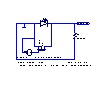
\includegraphics[width=60mm]{images/ltspice/jac/shortcircuit-transmitter.eps}
    \caption[\code{LTspice}-Schaltung Kurzschlussmethode, Sender, vereinfacht]{
        Simulationsschema  f\"ur  ein  einzelnes Modul  mit  kurzschliessendem
        Transistor und angeschlossener Last von \SI{1}{\kilo\ohm}.%
    }
    \label{fig:ltspice:shortCircuit:transmitter}
    \vspace*{-4em}
\end{wrapfigure}

Zuerst wird ein vereinfachtes Szenario simuliert: Ein einzelnes Modul mit einem
kurzschliessenden Transistor und einer Ohm'schen Last, dargestellt in Abbildung
\ref{fig:ltspice:shortCircuit:transmitter}.


\begin{figure}[h!tb]
    \begin{tikzpicture}
    \begin{scope}[x={(0mm,0.95\textwidth)},y={(0mm,150mm)}]
        \begin{axis}[%
            title=Spannung am Knoten \code{MEASURE},
            height=45mm,
            width=0.95\textwidth,
            at={(0,100mm)},
            grid=both,
            xlabel=Zeit (\si{\micro\second}),
            ylabel=Spannung (\si{\volt}),
            xmin = 0,
            xmax = 2e-4,
            change x base=true,
            x SI prefix=micro,
        ]
            \addplot[-,blue] table[x=time, y=V(measure)] {data/short-circuit/shortcircuit-transmitter-0.2ms.dat};
        \end{axis}
        \begin{axis}[%
            title=Strom durch MOSFET und Modul,
            height=45mm,
            width=0.95\textwidth,
            at={(0,50mm)},
            grid=both,
            xlabel=Zeit (\si{\micro\second}),
            ylabel=Strom (\si{\ampere}),
            xmin = 0,
            xmax = 2e-4,
            change x base=true,
            x SI prefix=micro,
        ]
            \addplot[-,blue] table[x=time, y=Id(MOS)] {data/short-circuit/shortcircuit-transmitter-0.2ms.dat};
            \addplot[-,magenta] table[x=time, y=I(module)] {data/short-circuit/shortcircuit-transmitter-0.2ms.dat};
            \legend{MOSFET,PV-Modul};
        \end{axis}
        \begin{axis}[%
            title=Leistung im MOSFET und PV-Modul,
            height=45mm,
            width=0.95\textwidth,
            at={(0,0)},
            grid=both,
            xlabel=Zeit (\si{\micro\second}),
            ylabel=Leistung (\si{\watt}),
            xmin = 0,
            xmax = 1.5e-6,
            change x base=true,
            x SI prefix=micro,
        ]
            \addplot[-,blue] table[x=time, y=powerMOS] {data/short-circuit/shortcircuit-transmitter-PPeak.dat};
            \addplot[-,magenta] table[x=time, y=powerModule] {data/short-circuit/shortcircuit-transmitter-PPeak.dat};
            \legend{MOSFET,PV-Modul};
        \end{axis}
   \end{scope}
\end{tikzpicture}

    \caption[Simulationsergebnisse Kurzschlussmethode, Sender]{%
        Transientensimulation    f\"ur     einen    gesteuerten    Kurzschluss
        \"uber     ein     Solarmodul     mit     einer     rein     Ohm'schen
        Last      von      \SI{100}{\ohm}     gem\"ass      der      Schaltung
        in   Abbildung   \ref{fig:ltspice:shortCircuit:transmitter}. Positives
        Vorzeichen bedeutet aufgenommene Leistung (also thermische Verluste).%
    }
    \label{fig:simu:shortCircuit:transmitter}
\end{figure}


Wie  in Abbildung  \ref{fig:simu:shortCircuit:transmitter} sichtbar,  kommt am
Knoten \code{MEASURE} ein  recht klares Signal an. Der Strom  durch den MOSFET
oszilliert bei durchgeschaltetem  Transistor ungef\"hart um den  im Mittel vom
Modul angegebenen Strom. Auffallend sind  die Spannungs- und Leistungsspitzen,
welche beim Deaktivieren des  Transistors auftreteten. Das PV-Modul gibt f\"ur
kurze  Zeit  sogar  beinahe  \SI{600}{\watt}  ab  und  der  MOSFET  absorbiert
mehr  als \SI{400}{\watt},  allerdings sind  diese Spitzen  sehr kurz  und die
thermischen Verluste im  Transistor sind im Mittel bei  einem Sendevorgang von
\SI{1}{\milli\second} lediglich etwa \SI{1}{\watt}.


% ---------------------------------------------------------------------------- %
\clearpage
\subsection{\Master~(Empf\"anger)}
\label{subsec:simu:ask:recv}
% ---------------------------------------------------------------------------- %

Die  Empf\"angerschaltung basiert  auf  dem  Prinzip der  Klemmenschaltung. Es
existieren verschiedene Implementationen; die  hier gew\"ahlte ist schematisch
in Abbildung \ref{fig:circuit:clamper} dargestellt. Der Zweck dieser Schaltung
ist, den DC-Anteil  aus dem ankommenden Signal auszukoppeln und  den Pegel des
verbleibenden  AC-Signals in  definierte  Grenzen zu  konvertieren, sodass  es
anschliessend  in die  Empf\"angerschaltung weitergeleitet  werden kann,  ohne
diese zu besch\"adigen.

Im vorliegenden Fall  muss die Klemmenschaltung die  Spannungsabf\"alle in der
Gr\"ossenordnung  von  einigen  Dutzend  Volt  (ein  kurzschliessendes  Modul)
ausfiltern  und  anschliessend  auf  ein  Signal  zwischen  \SI{0}{\volt}  und
\SI{3.3}{\volt}  konvertieren, welches  dann vom  Empf\"anger ohne  Gefahr von
Sch\"aden ausgewertet werden kann.

\begin{figure}[h!tb]
    \centering
    \begin{circuitikz}
    \small

    \draw
    (-1,0) node[ocirc] {\hspace*{-1.5em}IN} -- (0,0)
    to[C,l^=$\mathrm{C_{in}}$]
    (1,0) to[R,l^=$\mathrm{R_{in}}$]
    (5,0) node[circ] { } --
    (7,0) node[circ] { } --
    (9,0) node[ocirc] {~~OUT};
    %(8,0) to[R,l^=$\mathrm{R_{out}}$] (11,0)

    \draw
    (5,0) to[empty Zener diode,l_=D1] (5,2) --
    (7,2) to[R,l^=$\mathrm{R_{pull-up}}$]
    (7,0);

    \draw
    (7,0) to[R,l^=$\mathrm{R_{pull-down}}$]
    (7,-2) --
    (5,-2) to[empty Zener diode,l_=D2] (5,0);

    \draw
    (6,-2) node[circ] { } -- (6,-2.5) node[ocirc] {~~$\mathrm{V_{low}}$};

    \draw
    (6,2) node[circ] { } -- (6,2.5) node[ocirc] {~~$\mathrm{V_{high}}$};
\end{circuitikz}

    \caption[Klemmenschaltung]{Die hier verwendete Klemmenschaltung}
    \label{fig:circuit:clamper}
\end{figure}

Das Funktionsprinzip ist dabei wie folgt:

\begin{itemize}
    \tightlist
    \item
        $\mathrm{C_{in}}$ koppelt das AC-Signal aus  der Leitung aus (ist also
        ein sehr einfacher Hochpassfilter).
    \item
        $\mathrm{R_{in}}$ begrenzt den Strom,  welcher in die Klemmenschaltung
        fliesst, sollte also hochohmig sein.
    \item
        $\mathrm{R_{pull-up}}$  und  $\mathrm{R_{pull-down}}$ sorgen  daf\"ur,
        dass  die   Spannung  auf  dem  mittleren   Schaltungsabschnitt  immer
        definiert ist.
    \item
        $\mathrm{V_{high}}$  und  $\mathrm{V_{low}}$  sind  die  gew\"unschten
        obere  respektive untere  Pegelgrenze des  Ausgangssignals. In unserem
        Fall sind dies \SI{3.3}{\volt} und \SI{0}{\volt} bzw. \code{Ground}.
    \item
        Die   beiden  Dioden   D1   und  D2   sind  Zener-Dioden. Steigt   die
        Spannung  am Ausgang  auf einen  Wert, der  \"uber $\mathrm{V_{low}  +
        V_{breakdown,D2}}$ liegt, wird die Diode D2 durchbrechen. Somit steigt
        die Spannung nicht \"uber den durch die untere Klemmenspannung und die
        Durchbruchspannung  der  Diode  definierten Wert. Sinkt  die  Spannung
        zwischen  am  Ausgang  unter $\mathrm{V_{high}  -  V_{breakdown,D1}}$,
        bricht die obere Diode durch, womit ein Minimalwert f\"ur die Spannung
        am Ausgang definiert ist.
\end{itemize}

Zur   Simulation  wird   in   \code{LTspice}  die   Schaltung  aus   Abbildung
\ref{fig:ltspice:shortCircuit:receiver}  benutzt. Einige Simulationsergebnisse
sind in  Abbildung \ref{fig:simu:short:recv} dargestellt. Es wird  sowohl ohne
Last  wie auch  mit  Ohm'sch-kapazitiver  Last simuliert. Eine  abgesch\"atzte
Leitungsimpedanz von  \SI{100}{\micro\henry} ist  ebenfalls in  die Simulation
integriert.

\begin{figure}[h!tb]
    \centering
    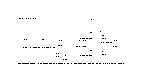
\includegraphics[width=\textwidth]{images/ltspice/jac/shortcircuit-recv.eps}
    \caption[\code{LTspice}-Schema f\"ur Klemmenschaltung]{
        Simulationsschema f\"ur die Simulation  der Klemme am Empf\"anger.%
    }
    \label{fig:ltspice:shortCircuit:receiver}
\end{figure}

Abbildung \ref{fig:ltspice:shortCircuit:receiver} zeigt die \code{LTspice}-Schaltung,
welche zur Simulation benutzt wird.
Das ankommende  Signal  wird  durch   einen  negativen  Spannungspuls  von
\SI{-45}{\volt}   am   Eingang   simuliert   (Leerlaufspannung   eines
PV-Moduls),  welche  die  ankommende DC-Spannung  von  \SI{900}{\volt}
einbrechen   l\"asst. In der Leitung ist eine parasit\"are Induktivit\"at
von \SI{100}{\micro\henry} eingebaut

Ebenfalls gezeigt  ist eine  Ohm'sch-kapazitive Last von  \SI{1}{\kilo\ohm} ||
\SI{100}{\micro\farad}. Die  Simulationsergebnisse ohne  Last  sind im  oberen
Plot in  Abblidung \ref{fig:simu:short:recv} gezeigt;  der untere Plot  in der
gleichen Abbildung  zeigt das  simulierte Verhalten der  Schaltung mit  der in
Abbildung \ref{fig:ltspice:shortCircuit:receiver} gezeigten Last.

Auf  der  rechten  Seite  ist   ein  Pull-down  Widerstand  auf  \code{Ground}
eingebaut,  um einen  definierten  Signalpegel zu  haben. Dies  ist f\"ur  die
Simulation notwendig, geh\"ort aber nicht per se zur Klemmenschaltung.

\clearpage
\begin{figure}[h!tb]
    \centering
    \begin{tikzpicture}
    \begin{scope}[x={(0mm,0.95\textwidth)},y={(0mm,100mm)}]
        \begin{axis}[%
            title=Klemmenschaltung Spannung am Empf\"anger{,} ohne Last,
            height=45mm,
            width=0.95\textwidth,
            at={(0,50mm)},
            grid=both,
            xlabel=Zeit (\si{\milli\second}),
            ylabel=Spannung (\si{\volt}),
            change x base=true,
            x SI prefix=milli,
            xmin = 0,
            xmax = 3e-4,
            %yticklabel={\num[round-mode=places, round-precision=4]{\tick}},
        ]
        \addplot[-,blue] table[x=time, y=V(receiver)] {data/short-circuit/shortcircuit-recv--noload.dat};
            %\addplot[-,magenta] table[x=time, y=powerModule] {data/short-circuit/shortcircuit-transmitter-PPeak.dat};
            %\legend{MOSFET,PV-Modul};
        \end{axis}
        \begin{axis}[%
            title=Klemmenschaltung Spannung am Empf\"anger{,} Last: \SI{1}{\kilo\ohm}{,} \SI{100}{\micro\farad},
            height=45mm,
            width=0.95\textwidth,
            at={(0,0)},
            grid=both,
            xlabel=Zeit (\si{\second}),
            ylabel=Spannung (\si{\volt}),
            xmin = 0,
            xmax = 5,
            %change x base=true,
            %x SI prefix=micro,
            %yticklabel={\num[round-mode=places, round-precision=4]{\tick}},
        ]
        \addplot[-,blue] table[x=time, y=V(receiver)] {data/short-circuit/shortcircuit-recv--1kohm100uF--10s.dat};
            %\addplot[-,magenta] table[x=time, y=powerModule] {data/short-circuit/shortcircuit-transmitter-PPeak.dat};
            %\legend{MOSFET,PV-Modul};
        \end{axis}
   \end{scope}
\end{tikzpicture}

    \caption[Simulationsergebnisse Klemmenschaltung]{%
        Simulation   Empf\"anger. Die   obere   Kurve  ist   das   Signal   am
        Empf\"anger  ohne  angeschlossene Last. Der  \"Ubertragungsvorgang  im
        unteren  Bild beginnt  bei einer  Sekunde. Die Schaltungsfrequenz  ist
        \SI{10}{\kilo\hertz}%
    }
    \label{fig:simu:short:recv}
\end{figure}

Wie  an  Abbildung  \ref{fig:simu:short:recv}  gesehen werden  kann,  hat  die
Art  der  angeh\"angten Last  einen  merklichen  Einfluss auf  das  ankommende
Signal. Ein grosser kapazitiver Anteil in der Last reduziert die Amplitude des
ankommenden  Signals  bedeutend und  f\"uhrt  einen  sehr lange  (etwa  f\"unf
Sekunden!) dauernden Entlade- und Ladevorgang der kapazitiven Anteile im Kreis
ein.


% ---------------------------------------------------------------------------- %
\clearpage
\subsection{Gesamtsystem}
\label{subsec:simu:ask:total}
% ---------------------------------------------------------------------------- %


Im  Folgenden   werden  der  oben  untersuchte   Transmitter  und  Empf\"anger
in  den  bereits  in  Abschnitt  \ref{sec:simu:model:module:string}  ab  Seite
\pageref{sec:simu:model:module:string}   vorgestellten   Modulstrang  aus   20
Modulen  mit  einer  \SI{20}{\meter} langen  Anschlussleitung  (pro  Richtung)
eingebaut und das Verhalten des Gesamtsystems untersucht.

Die zugeh\"orige  Simulationsschaltung f\"ur  \code{LTspice} ist  in Abbildung
\ref{fig:ltspice:shortcircuit:complete} dargestellt.

\begin{figure}[h!tb]
    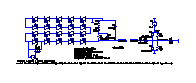
\includegraphics[width=\textwidth]{images/ltspice/jac/shortcircuit.eps}
    \caption[\code{LTspice}-Schaltung f\"ur Kurzschlussmethode, Modulstrang]
    {Gesamte Simulationsschaltung f\"ur die Kurzschlussmethode}
    \label{fig:ltspice:shortcircuit:complete}
\end{figure}

\begin{figure}[h!tb]
    \centering
    \begin{tikzpicture}
    \begin{scope}[x={(0mm,0.95\textwidth)},y={(0mm,110mm)}]
        \begin{axis}[%
            title=Klemmenschaltung Spannung am Empf\"anger{,} \code{Rload} {=} \SI{1}{\kilo\ohm},
            height=50mm,
            width=0.95\textwidth,
            at={(0,55mm)},
            grid=both,
            xlabel=Zeit (\si{\micro\second}),
            ylabel=Spannung (\si{\volt}),
            change x base=true,
            x SI prefix=micro,
            legend cell align = left,
            xmin = 0,
            xmax = 3e-4,
            %yticklabel={\num[round-mode=places, round-precision=4]{\tick}},
        ]
        %\addplot[-,blue] table[x=time, y=V(receiver)] {data/short-circuit/shortcircuit-Cload-steps.dat};
        \addplot[-,blue] table[x=time, y=V(receiver)] {data/short-circuit/shortcircuit-Cload-1n.dat};
        %\addplot[-,magenta] table[x=time, y=V(receiver)] {data/short-circuit/shortcircuit-Cload-10n.dat};
        \addplot[-,cyan] table[x=time, y=V(receiver)] {data/short-circuit/shortcircuit-Cload-100n.dat};
        %\addplot[-,purple] table[x=time, y=V(receiver)] {data/short-circuit/shortcircuit-Cload-1u.dat};
        \addplot[-,solarized-magenta] table[x=time, y=V(receiver)] {data/short-circuit/shortcircuit-Cload-10u.dat};
        \legend{%
            $\mathrm{C_{load}} = \SI{1}{\nano\farad}$,
            $\mathrm{C_{load}} = \SI{100}{\nano\farad}$,
            $\mathrm{C_{load}} = \SI{1000}{\nano\farad}$%
        };
            %\addplot[-,magenta] table[x=time, y=powerModule] {data/short-circuit/shortcircuit-transmitter-PPeak.dat};
            %\legend{MOSFET,PV-Modul};
        \end{axis}
        \begin{axis}[%
            title=Klemmenschaltung Spannung am Empf\"anger{,} \code{Cload} {=} \SI{100}{\nano\farad},
            height=50mm,
            width=0.95\textwidth,
            at={(0,0)},
            grid=both,
            xlabel=Zeit (\si{\micro\second}),
            ylabel=Spannung (\si{\volt}),
            change x base=true,
            x SI prefix=micro,
            legend cell align = left,
            xmin = 0,
            xmax = 3e-4,
            %yticklabel={\num[round-mode=places, round-precision=4]{\tick}},
        ]
        %\addplot[-,blue] table[x=time, y=V(receiver)] {data/short-circuit/shortcircuit-Rload-10.dat};
        \addplot[-,blue] table[x=time, y=V(receiver)] {data/short-circuit/shortcircuit-Rload-100.dat};
        \addplot[-,cyan] table[x=time, y=V(receiver)] {data/short-circuit/shortcircuit-Rload-1k.dat};
        \addplot[-,solarized-magenta] table[x=time, y=V(receiver)] {data/short-circuit/shortcircuit-Rload-10k.dat};
        \legend{%
            %$\mathrm{R_{load}} = \SI{10}{\ohm}$,
            $\mathrm{R_{load}} = \SI{100}{\ohm}$,
            $\mathrm{R_{load}} = \SI{1}{\kilo\ohm}$,
            $\mathrm{R_{load}} = \SI{10}{\kilo\ohm}$%
        };
            %\addplot[-,magenta] table[x=time, y=powerModule] {data/short-circuit/shortcircuit-transmitter-PPeak.dat};
            %\legend{MOSFET,PV-Modul};
        \end{axis}
   \end{scope}
\end{tikzpicture}

    \caption[Simulationsergebnisse Kurzschlussmethode]{%
        Simulationsergebnisse  f\"ur  das  Signal  am  Knoten  \code{RECEIVER}
        aus  Abbildung  \ref{fig:ltspice:shortcircuit:complete}  f\"ur  Lasten
        mit   verschiedenen    kapazitiven   Anteilen    \code{Cload}   (obere
        Plots)  und  resistiven   Anteilen  \code{Rload}  (untere  Plots). Die
        \"Ubertragungsfrequenz betr\"agt \SI{10}{\kilo\hertz}.%
    }
    \label{fig:simu:short:complete}
\end{figure}

Wie   in   Abbildung   \ref{fig:simu:short:complete}   zu   sehen,   hat   die
angeschlossene Last einen  betr\"achtlichen Einfluss auf das  Signal (wie auch
schon im vorigen Abschnitt  beobachtet), welches beim Empf\"anger ankommt. Bei
einem Ohm'schen Lastwiderstand von \SI{1}{\kilo\ohm} und einer Lastkapazit\"at
von  bereits \SI{100}{\nano\farad}  kommt  anstatt  eines Rechteckpulses  eine
Doppelschwingung beim  Empf\"anger an;  steigt die Gr\"osse  der parasit\"aren
Komponente der  Last auf \SI{1}{\milli\farad},  ist vom Signal  am Empf\"anger
bei der eingestellten Frequenz nicht mehr viel zu sehen.

Auch die  Ohm'sche Komponente der  Last hat  bedeutenden Einfluss; ist  sie zu
klein, sinkt die Signalamplitude am  Empf\"anger stark (blaue Kurve im unteren
Plot von Abbildung \ref{fig:simu:short:complete}).

Die Gesamtbeurteilung  dieses Ansatzes  ist gemischt: Prinzipiell  k\"onnte es
m\"oglich sein, eine  funktionierende Implementation zu entwickeln. Allerdings
gibt  es  Faktoren,  welche  erhebliche Auswirkungen  auf  die  Erfolgschancen
aus\"uben k\"onnen, und  auf die wir keinen Einfluss haben,  oder deren genaue
Untersuchung im Rahmen  dieses Projekts aus Zeit-  und Materialgr\"unden nicht
m\"oglich ist.

Sollte   diese   L\"osungsvariante   implementiert  werden,   m\"ussten   noch
detaillierte Untersuchungen  gemacht werden. Nicht nur muss  das Verhalten des
PV-Moduls (bzw. des Modulstrangs) bekannt  sein, es m\"ussen auch detaillierte
Informationen \"uber die angeh\"angten  Lasten eingeholt werden.  Insbesondere
muss das  Verhalten des  Wechselrichters unter  verschiedenen Betriebsbedingen
(Last, momentane Leistung der PV-Modulstr\"ange, allenfalls weitere unbekannte
Parameter)  bekannt sein. Abh\"angig  von  den  Charakteristiken der  gesamten
mit  dem  Modulstrang  verbundenen  Schaltung k\"onnte  es  sein,  dass  diese
L\"osungsvariante nicht implementierbar ist. Oder es m\"ussten m\"oglicherwise
weitere Schaltkreise entwickelt und eingebaut werden, um mit dem Verhalten des
Wechselrichters  und  den  an  ihn angeh\"angten  Lasten  korrekt  umgehen  zu
k\"onnen. Dies wiederum  w\"are nicht  wirklich im  Sinne dieser  L\"osung, da
ihre grosse Attraktivit\"at  genau darin liegen w\"urde,  dass ihr Schaltungs-
und Materialaufwand (theoretisch) sehr gering ist.

Grunds\"atzlich finden wir diese  L\"osungsvariante aufgrund des enorm simplen
Prinzips zwar sehr interessant. Da dies  jedoch (soweit uns bekannt) absolutes
Neuland ist und wir die Ressourcen  nicht haben, um einen Modulstrang oder das
an einen Modulstrang  angeh\"angte System wirklich genau  zu untersuchen (also
ausmessen statt  lediglich simulieren),  beurteilen wir die  Erfolgschancen im
Rahmen eines Semesterprojekts f\"ur diese Methode als zu gering, um sie weiter
zu verfolgen.


% ---------------------------------------------------------------------------- %
\clearpage
\section{Schlussfolgerungen}
\label{subsec:simu:conclusion}
% ---------------------------------------------------------------------------- %

Es folgt  an dieser  Stelle eine  zusammenfassende Gegen\"uberstellung  der in
den vorigen  Abschnitten untersuchten  L\"osungsvarianten und  ein Entschluss,
welche Variante weshalb weiterverfolgt wird. Tabelle \ref{tab:simu:conclusion}
enth\"alt eine \"Ubersicht einiger Merkmale der verschiedenen Ans\"atze.

Die Kurzschlussvariante  wird aufgrund der starken  Lastabh\"angigkeit und der
Neuartigkeit des  Konzepts nicht weiterverfolgt. Wie bereits  angemerkt halten
wird  diesen  Ansatz  zwar  f\"ur sehr  interessant,  beurteilen  aber  unsere
Erfolgschancen  im  Rahmen eines  Semesterprojekts  als  zu gering,  um  diese
Variante weiter zu verfolgen.

Bei der  kapazitiven Einkopplung hat  der Ort, an  dem die Einkopplung  in den
Strang erfolgt einen  grossen Einfluss nicht nur auf  die Signalamplitude beim
Empf\"anger, sondern auf die Form  des Signals. Dies beurteilen wird als nicht
optimal, da allenfalls  komplexe L\"osungen n\"otig w\"aren, um  das Signal am
Empf\"anger \"uberhaupt noch als solches erkennen zu k\"onnen.

Aufgrund der niedrigen  Verzerrung des Signals bei  der induktiven Einkopplung
wird diese  Variante implementiert. Die Signalamplitude beim  Betrieb in einem
Strang mit mehreren Modulen kann zwar  stark abfallen, jedoch ist selbst unter
diesen  Umst\"anden  das Signal  prinzipiell  noch  sehr sauber  und  k\"onnte
allenfalls wieder herausgefiltert  und verst\"arkt werden. Alternativ k\"onnte
in einer weiteren Entwicklungsstufe eine L\"osung implementiert werden, welche
den Strang, in  dem ein Sensor installiert ist, ausmisst,  und automatisch bei
der  optimalen Frequenz  (innerhalb  von  spezifizierten Grenzen  nat\"urlich)
sendet.

\begin{table}[h!tb]
    \centering
    \small
    \caption{Gegen\"uberstellung der drei L\"osungsvarianten}
    \label{tab:simu:conclusion}
    \begin{tabular}{p{38mm}p{28mm}p{28mm}p{28mm}}
        \toprule
        \textbf{Kriterium} &
        \textbf{induktive Kopplung} &
        \textbf{kapazitive Kopplung} &
        Kurzschluss \\

        \midrule

        Komplexit\"at der Schaltung &
        mittel &
        mittel &
        simpel \\
        [2mm]

        \rowcolor{solarized-base2}
        Neuartigkeit des Konzepts &
        niedrig &
        niedrig &
        hoch \\
        [2mm]

        Kosten &
        hoch &
        mittel &
        klein  \\
        [2mm]

        \rowcolor{solarized-base2}
        St\"arke des Signals am Empf\"anger &
        bei Resonanz gut, kann sonst stark abfallen &
        variiert stark mit Position im Strang &
        variiert stark mit Last \\
        [2mm]

        Verzerrung des Signals am Empf\"anger &
        schwache Verzerrung &
        variiert mit Position im Strang, Signal kann sehr stark verzerrt werden &
        variiert stark mit Last \\
        \bottomrule
    \end{tabular}
\end{table}
